\chapter{RESULTS AND DISCUSSION}
\label{ch:results}
\section{Introduction}
This chapter evaluates the performance of machine learning (baseline) and hybrid deep learning models in predicting malaria risk across Kenya's 47 counties using data from 2016 to 2025. Following exploratory data analysis (EDA), assesing model accuracy using $RMSE$, $MAE$, and $R^2$ metrics. Then concludes with spatial malaria risk mapping and comparison evaluation of predictive model performance.

\section{Descriptive Statistics }
\subsection{Dataset Overview}
   The study utilized 5,640 county-month observations integrating climatic, environmental, demographic, and intervention variables collected across Kenya's 47 counties between 2016 and 2025. Data validation  and data entry rules  were confirmed and completeness with no missing values or duplicates, ensuring a reliable foundation for predictive modeling.
   
    Table \ref{tab:hotspot_data_structure} Shows hotspot counties and Lamu  exhibited relatively high malaria incidence despite having a smaller population size compared to Kisumu and Homa Bay. We can clearly see that environmental suitability, rather than population size alone, plays a major role in malaria transmission dynamics. 
\begin{table}[H]
	\centering
	\caption{Example Records from High-Risk Malaria Hotspot Counties}
	\label{tab:hotspot_data_structure}
	\small
	\begin{tabular}{lcccccccc}
		\hline
		County & Date & Rainfall & Temp & Humidity & NDVI & Population & Cases & Incidence \\
		\hline
		Kisumu & 2019-04 & 214.62 & 26.84 & 84.71 & 0.76 & 1,155,574 & 356 & 0.3081 \\
		Homa Bay & 2019-04 & 228.31 & 27.15 & 86.42 & 0.79 & 1,131,950 & 331 & 0.2924 \\
		Lamu & 2019-04 & 198.75 & 28.63 & 82.53 & 0.71 & 143,920 & 58 & 0.4030 \\
		\hline
	\end{tabular}
\end{table}

\subsection{Summary Statistics}

Table \ref{tab:summary_stats} presents the description of statistics of the major  variables.

\begin{table}[H]
	\centering
	\caption{Summary Statistics of Major Study Variables}
	\label{tab:summary_stats}
	\begin{tabular}{lcccc}
		\hline
		Variable & Mean & Std. Dev & Minimum & Maximum \\
		\hline
		Rainfall (mm) & 119.24 & 68.43 & 2.27 & 574.32 \\
		Temperature ($^\circ$C) & 24.98 & 2.01 & 17.73 & 31.36 \\
		Humidity (\%) & 75.14 & 8.68 & 60.01 & 89.98 \\
		NDVI & 0.55 & 0.14 & 0.30 & 0.80 \\
		Population & 1,064,621 & 725,757.30 & 133,189 & 5,137,957 \\
		ITN Coverage & 0.60 & 0.11 & 0.40 & 0.80 \\
		IRS Coverage & 0.30 & 0.12 & 0.10 & 0.50 \\
		Treatment Coverage & 0.70 & 0.12 & 0.50 & 0.90 \\
		Incidence per 1000 & 0.0175 & 0.0217 & 0.0000 & 0.3998 \\
		\hline
	\end{tabular}
\end{table}
Table \ref{tab:summary_stats} illustrates major environmental and climatic variances among Kenyan counties. Temperature and humidity were different across location and season, with rainfall ranging from 2.27 mm to 574.32 mm.  The environmental differences match the observed variation in malaria incidence among counties. The use of nonlinear machine learning and hybrid deep models for malaria prediction is supported by significant variation in both environmental circumstances and malaria incidence.
\begin{figure}[htbp]
   Figure \ref{fig:env_variables} presents the EDA analysis of malaria incidence and environmental variables across Kenya from 2016 to 2025. We conducted the  analysis to examine spatial variability, temporal trends, and environmental relationships before predictive model development.
	\centering
	
	\begin{minipage}[t]{0.48\textwidth}
		\centering
		\includegraphics[width=\linewidth]{COUNTY INCIDENCE COMPARISON.png}
		\caption*{(a) Spatial Distribution of Malaria Incidence Across Counties}
		
		\vspace{0.2cm}
		
	  \small Based on the study, Figure 4.1(a) clearly illustrates the spatial variations in malaria incidence  among Kenyan counties. Compared to numerous central counties, Kisumu, Lamu, and Isiolo had higher malaria incidence and greater fluctuations. The spatial variance suggests that localized climatic and environmental factors covered in Section~\ref{sec:study_area} have significant impact on malaria transmission. 
		
	\end{minipage}
	\hfill
	\begin{minipage}[t]{0.48\textwidth}
		\centering
		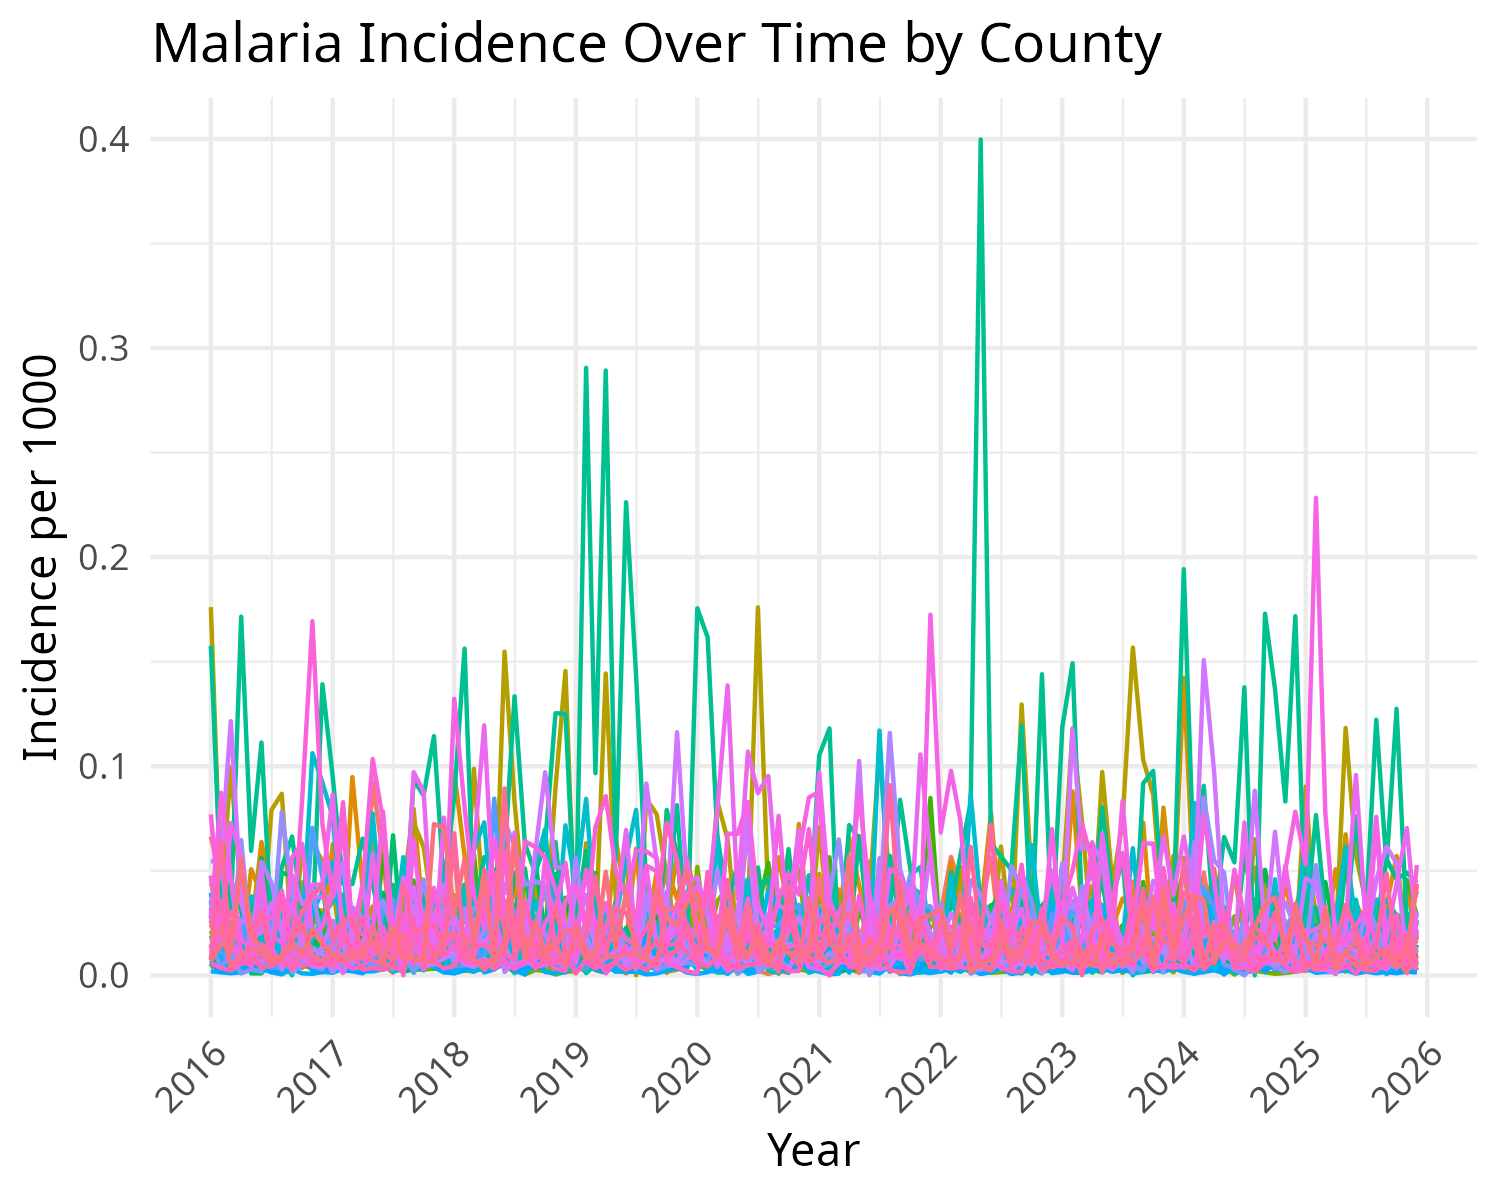
\includegraphics[width=\linewidth]{Temporal trends.png}
		\caption*{(b) Temporal Trends of Malaria Incidence Across Counties (2016--2025)}
		
		\vspace{0.2cm}
		
		\small Figure 4.1(b) illustrates temporal fluctuations in malaria incidence across counties from 2016 to 2025.  Due to delayed climate influences and temporal dependencies in malaria transmission,  several counties experienced seasonal outbreak peaks during specific periods.  We can tell temporal patterns support the lagged feature engineering method outlined   in subsection~\ref{sec:lagged_features}.
	\end{minipage}
	
	\vspace{0.5cm}
	
	\begin{minipage}[t]{0.48\textwidth}
		\centering
		\includegraphics[width=\linewidth]{Variables comparison.png}
		\caption*{(c) Comparison of Environmental Variables}
		
		\vspace{0.2cm}
		
		\small 
		The distribution of temperature, humidity,rainfall, and NDVI variables used in model performance development  shown in Figure 4.1(c). Among the climatic factors, rainfall had the greatest variability, suggesting significant variations in climate between counties and seasons. The use of machine learning and hybrid learning models can learn nonlinear environmental interactions.	
	\end{minipage}
	\hfill
	\begin{minipage}[t]{0.48\textwidth}
		\centering
		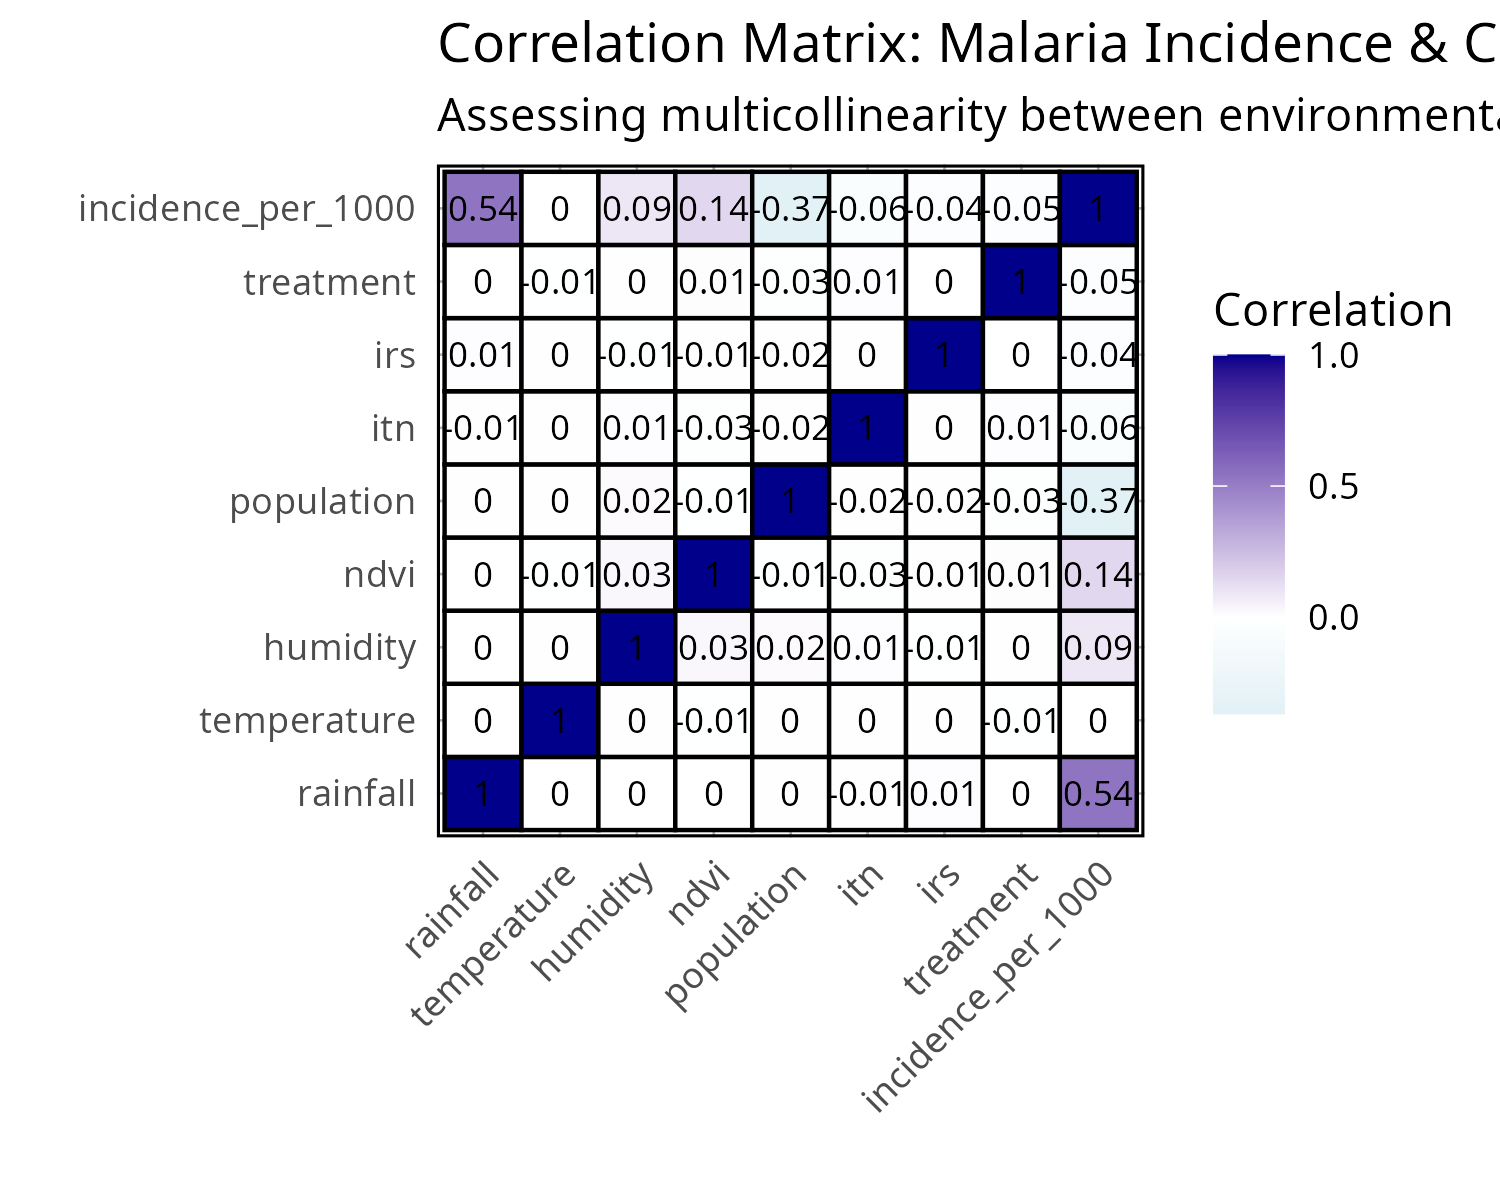
\includegraphics[width=\linewidth]{HEATMAP CORRELATION.png}
		\caption*{(d) Correlation Matrix of Malaria Incidence and Predictor Variables}
		
		\vspace{0.2cm}
		
		\small 	The correlation structure between predictor variables and malaria incidence is shown in Figure 4.1 (d). Rainfall had the strongest positive (\(r = 0.54\)) correlation with malaria incidence, while a number predictors had weak linear associations. This indicates that malaria transmission is influenced by complex nonlinear interactions, which validates the use of spatio-temporal learning models like CNN-LSTM and CNN-GRU  , covered in  Section~\ref{sec:hybrid_models}.
	\end{minipage}
	\caption{Exploratory Analysis of Malaria Incidence and Environmental Variables}
	\label{fig:env_variables}
	
\end{figure}

\FloatBarrier


\section{Comparison of Model Performance}

Table \ref{tab:model_results} compares the predictive performance of baseline machine learning and hybrid deep learning models metrics described in Section~\ref{sec:evaluation_metrics}.

\vspace{-0.2cm}
\begin{table}[H]
	\centering
	\caption{Performance Comparison of Machine Learning and Deep Learning Models}
	\label{tab:model_results}
	\small
	\begin{tabular}{lccc}
		\hline
		Model & RMSE & MAE & $R^2$ \\
		\hline
		XGBoost (Baseline) & 0.00863 & 0.00455 & 0.8199 \\
		Random Forest (Baseline) & 0.00972 & 0.00570 & 0.7718 \\
		LSTM & 0.010620 & 0.006413 & 0.7204 \\
		CNN-LSTM & 0.008764 & 0.005248 & 0.8096 \\
		CNN-GRU & 0.010146 & 0.006092 & 0.7448 \\
		CNN-Transformer & 0.014470 & 0.009105 & 0.4810 \\
		\hline
	\end{tabular}
\end{table}
 XGBoost attained the best overall predictive performance with an $R^2$ value of 0.8199, these indicated  that the model explained approximately 82\% of the variability in malaria incidence.  The model also recorded the lowest RMSE and MAE values, showing that its predictions were very close to the observed malaria incidence values. Its perfomance  suggests that ensemble tree-based learning effectively captured nonlinear interactions variables. Among the hybrid DL models, CNN-LSTM achieved the highest predictive performance with an $R^2$ value of 0.8096. The model outperformed standalone LSTM and CNN-GRU models, indicating that the integration of convolutional environmental  feature interaction and long-term temporal memory improved the representation of malaria transmission dynamics. This tells the importance of hybrid modelling spatial interactions and temporal dependencies. In contrast, The dataset from the county level may not have provided sufficient sequential complexity for the Transformer attention mechanism to learn stable long range temporal relationships making it have the weakest predictive performance.
 \begin{figure}[H]
 	\vspace{-0.3cm}
 	\subsection{Baseline ML Prediction Results}
 	Figure \ref{fig:baseline_ml} demonstrate that both ML models were able to capture the general malaria transmission patterns across Kenyan counties.
 	\centering
 	\includegraphics[width=0.82\textwidth,height=0.55\textheight,keepaspectratio]{Observed verse Predicted.png}
 	\caption{Observed vs Predicted Malaria Incidence for Baseline Machine Learning Models}
 	\label{fig:baseline_ml}
 \end{figure}
 We can see that XGBoost predictions clustered more closely around the perfect prediction line compared to RF, indicating lower prediction error and better predictive performance. This suggests that XGBoost was more effective in learning the complex nonlinear relationships associated with malaria transmission.  However, prediction variability increased slightly at higher malaria incidence levels, indicating that extreme outbreak periods were more difficult to predict accurately due to the complex nature of malaria transmission dynamics.
\section{Deep Learning Model Results}
Figure \ref{fig:dl_evaluation} presents the predictive performance of the hybrid deep learning models developed for malaria forecasting. The models were evaluated based on their ability to capture spatio-temporal malaria transmission patterns across counties and time periods.

\begin{figure}[H]
	\centering
	
	\begin{minipage}[t]{0.48\textwidth}
		\centering
		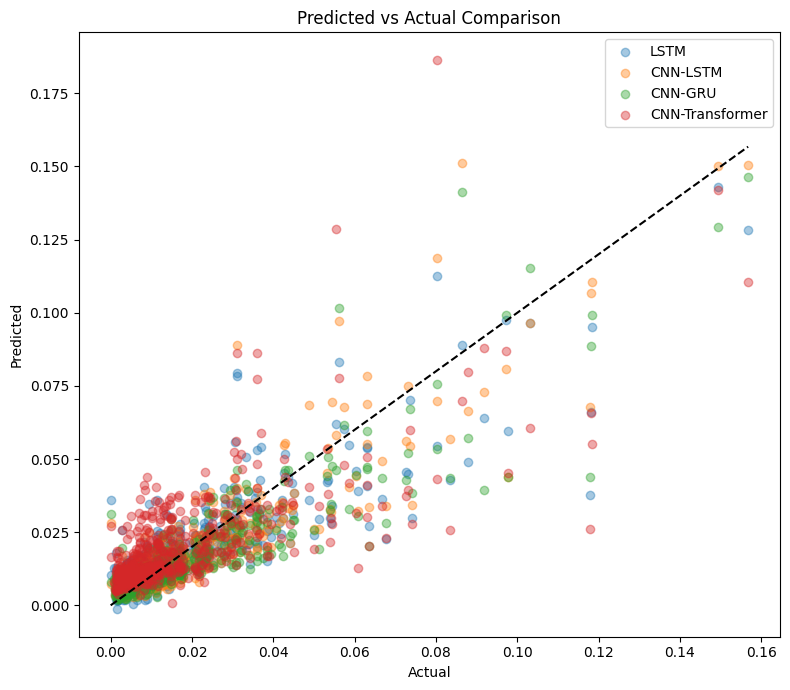
\includegraphics[width=\linewidth]{Predicted vs Actual.png}
		\caption*{(a) Predicted versus Actual Comparison}
	\end{minipage}
	\hfill
	\begin{minipage}[t]{0.48\textwidth}
		\centering
		\includegraphics[width=\linewidth]{Coefficient of models.png}
		\caption*{(b) Comparison of $R^2$ Scores}
	\end{minipage}
	
	\vspace{0.25cm}
	
	\begin{minipage}[t]{0.48\textwidth}
		\centering
		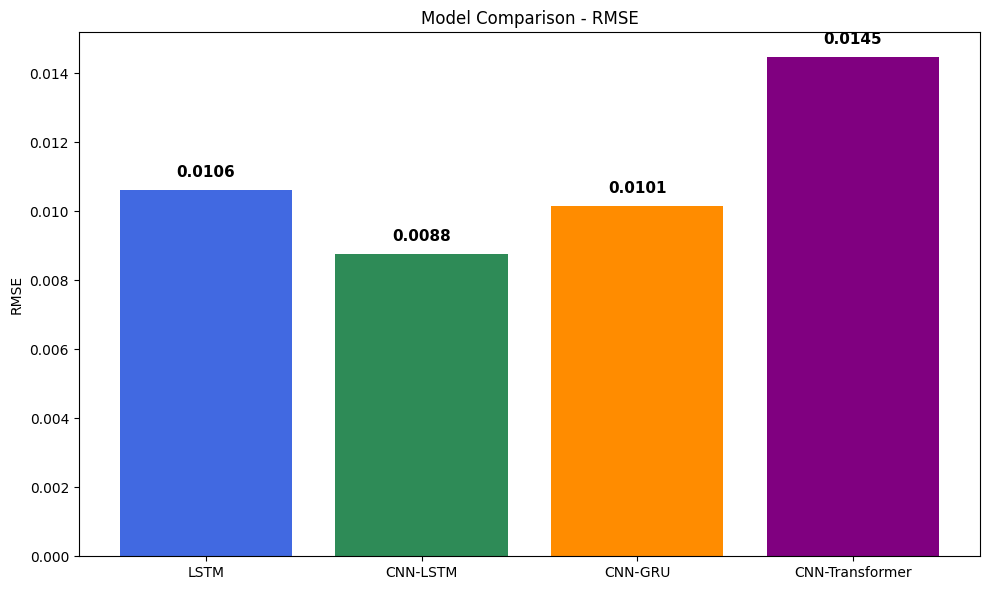
\includegraphics[width=\linewidth]{RMSE Comparison.png}
		\caption*{(c) Comparison of RMSE Values}
	\end{minipage}
	\hfill
	\begin{minipage}[t]{0.48\textwidth}
		\centering
		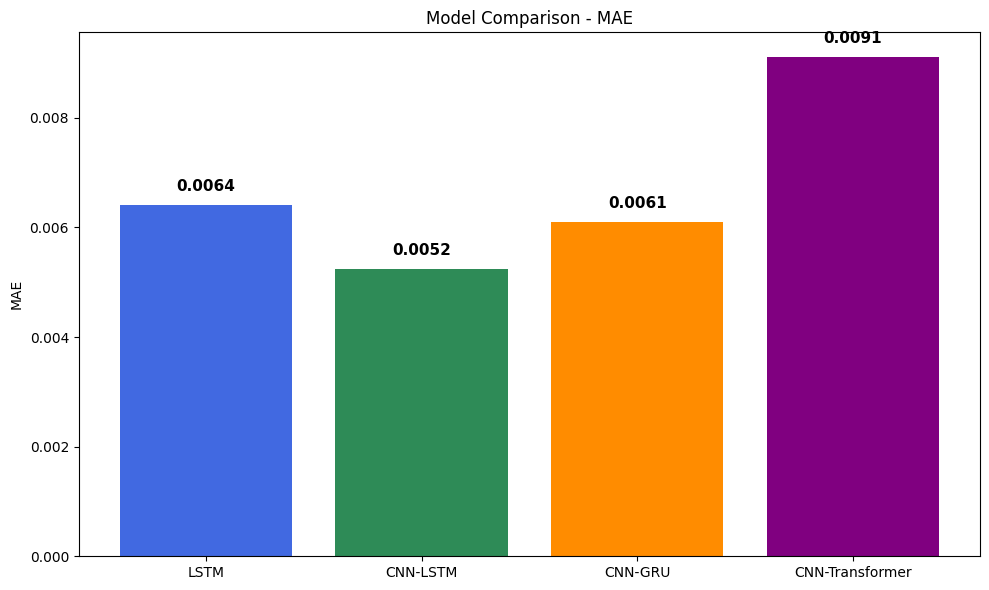
\includegraphics[width=\linewidth]{ MAE Comparison.png}
		\caption*{(d) Comparison of MAE Values}
		\end{minipage}
	\caption{Performance Evaluation of Deep Learning Models}
	\label{fig:dl_evaluation}
\end{figure}

\vspace{-0.2cm}
    From  the predicted versus actual plots, the CNN-LSTM predictions were more closely distributed around the diagonal reference line compared to the other models. We can see that the predicted malaria incidence values closely matched the observed data, showing strong prediction accuracy and consistency across different counties and time periods. Then CNN-Transformer displayed a much wider scatter of points especially at higher incidence levels which reveals larger prediction errors and a clear lack of stability when transmission rates increased.
    
    For the model performance, the hybrid CNN-LSTM model performed best among all tested models, achieving an RMSE of 0.0088, MAE of 0.0052, and an $R^2$ of 0.8096. Low error values tell us that the model's predictions remained highly accurate, successfully capturing both localized spatial variations and temporal transmission dynamics over the study period. This performance suggests that combining CNNs feature learning with temporal memory blocks significantly improves the capacity to represent complex nonlinear patterns of malaria risk, allowing the CNN layers to isolate environmental drivers such as rainfall, temperature, humidity, and vegetation while the LSTM component tracks lagging transmission effects and seasonal trends.The standalone LSTM model showed moderate performance, with an RMSE of 0.0106, MAE of 0.0064, and an $(R^2)$ value of 0.720. While it was able to capture the general temporal patterns in malaria transmission, its higher prediction errors compared to the hybrid models suggest that temporal information alone may not fully represent the spatial differences in malaria risk across counties.
    
    The CNN-GRU model showed slightly better results, yielding an RMSE of 0.0101, MAE of 0.0061, and an $R^2$ of 0.745. This indicates that while the GRU framework maintained relatively stable predictions and handled temporal dependencies , its lower accuracy compared to the CNN-LSTM implies that the explicit memory gating structure of LSTMs is better suited for retaining long-range transmission behavior and delayed climate impacts.
    
    The CNN-Transformer model presented the most challenging performance, recording the weakest with an RMSE of 0.0145, MAE of 0.0091, and an $R^2$ value of 0.481. These elevated error rates and the wide dispersion of its prediction points simply tell us that the model struggled to anchor onto stable transmission patterns at the county level, highlighting its unsuitability for shorter or less complex spatial sequences where self-attention mechanisms frequently generate noisy outputs. 
   \vspace{-0.5cm}
\begin{figure}[H]
	\centering
	\caption{Residual Analysis, Training Convergence, and County-monthly Forecasting Performance of the CNN-LSTM Model}
	\label{fig:cnnlstm_results}
	\hfill
	\begin{minipage}[t]{0.42\textwidth}
		\centering
		\includegraphics[width=\linewidth]{Residual Distribution.png}
		\caption*{(a) Residual Distribution Comparison}
		\end{minipage}
	\hfill
	\begin{minipage}[t]{0.50\textwidth}
		\centering
		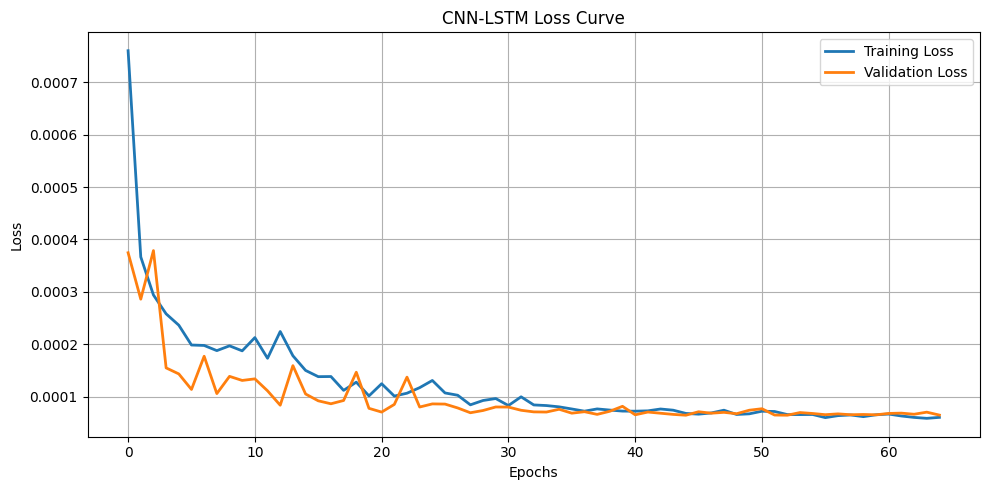
\includegraphics[width=\linewidth]{CNN-LSTM Loss Curve.png}
		\caption*{(b) CNN-LSTM Loss Curve}
	\end{minipage}
	\hfill
	\begin{minipage}[t]{0.60\textwidth}
		\centering
		\includegraphics[width=\linewidth]{Malaria Forecast Across Kenyan Counties.png}
		\caption*{(c) CNN-LSTM Forecast Across Selected Counties}
	\end{minipage}
	
	\vspace{-0.5cm}
	
	
\end{figure}

\vspace{-0.5cm}
\small Figure \ref{fig:cnnlstm_results}  above shows  prediction errors for the CNN-LSTM framework concentrated heavily around zero in the residual plots, showing relatively stable predictions with smaller overall forecasting errors across counties. Conversely, the CNN-Transformer produced a much broader error spread, reflecting diminished consistency when malaria transmission peaked.

During training, the CNN-LSTM loss curves demonstrated stable learning. Optimization occurred rapidly within the first 10 epochs, dropping from an initial training loss of 0.00075 and a validation loss of 0.00038 down to a flat floor of 0.00005 by epoch 20. The training and validation curves remained closely aligned throughout the training process without divergence through epoch 65. This close alignment suggests that the model generalized effectively without strong signs of overfitting despite the variability in climatic and malaria incidence data.

Regionally, the network mapped actual malaria pathways across vastly different ecological zones. In hyper-endemic Migori and Busia, it accurately traced seasonal peaks from 2020 to 2022, proving it successfully linked vector breeding cycles to heavy rainfall and temperature anomalies. For the arid landscape of Turkana County, the architecture traced major increases in malaria incidence associated with flooding periods, despite minor overpredictions at peak intensity. Similarly, along the coast in Lamu County, the model smoothly captured transmission fluctuations over the six-year window, confirming that the CNN-LSTM successfully balanced temporal disease rhythms with localized environmental traits. Furthermore ,
\begin{figure}[H]
	\small Figure \ref{fig:hybrid_dl_results} compares malaria incidence forecasts generated by the evaluated  Hybrid deep learning architectures. 
	\centering
	
	\begin{minipage}[t]{0.58\textwidth}
		\centering
		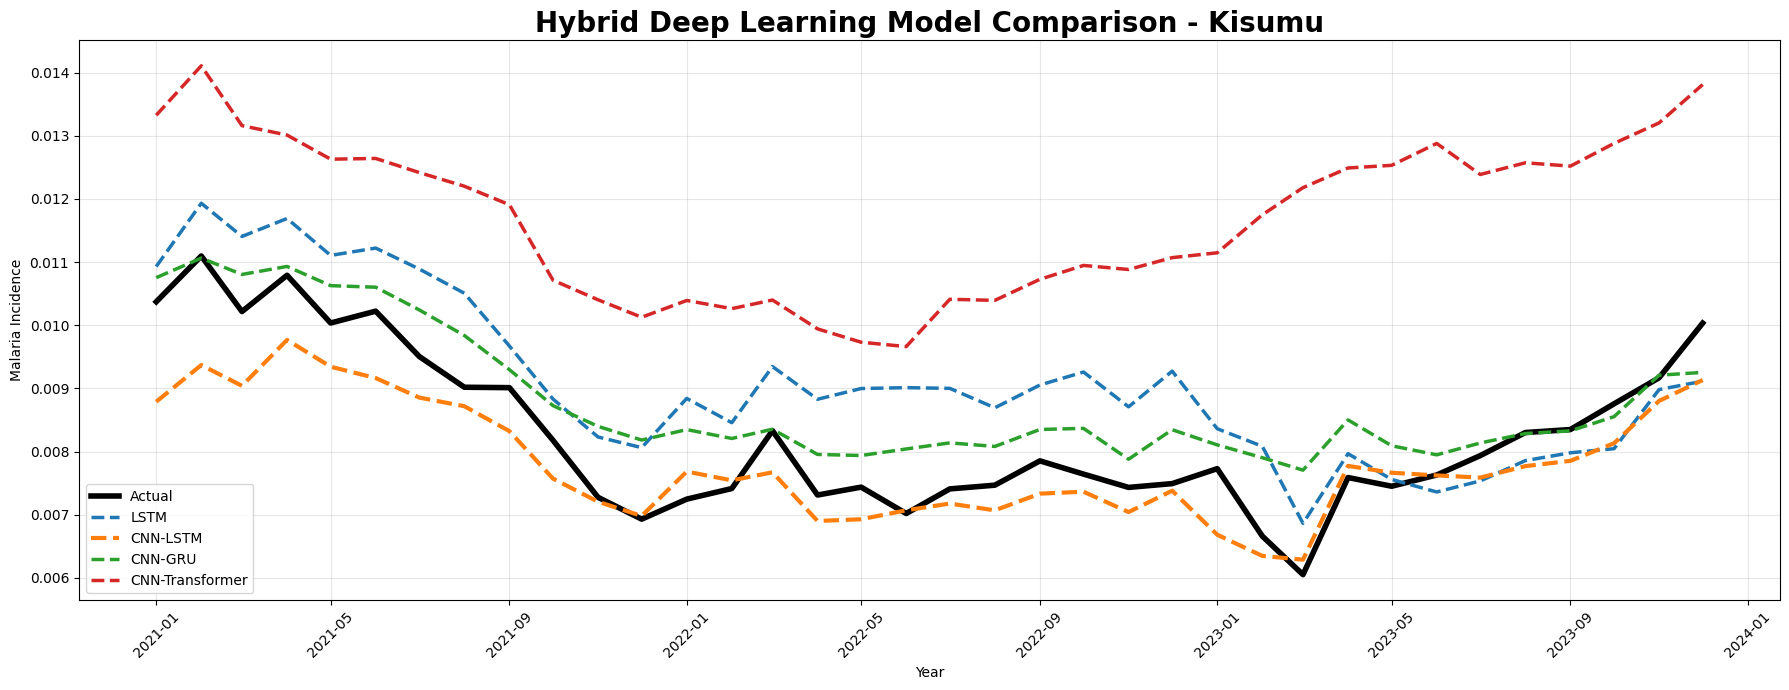
\includegraphics[width=\linewidth]{Hybrid Comparison.png}
		\caption*{(a) Hybrid Deep Learning Forecast Comparison}
	\end{minipage}
	\hfill
	\begin{minipage}[t]{0.38\textwidth}
		\centering
		\includegraphics[width=\linewidth]{Malaria Forecast Comparison.png}
		\caption*{(b) Malaria Forecast Comparison Across Deep Learning Models}
	\end{minipage}
	
	\vspace{-0.2cm}
	
	\caption{Comparative Deep Learning Forecasting Results}
	\label{fig:hybrid_dl_results}
\end{figure}

\vspace{-0.3cm}
Evaluating the Kisumu lake basin forecasts reveals clear performance disparities among the architectures. The hybrid CNN-LSTM network matched the real-world timeline best, capturing the major 2021 outbreak wave with minimal peak error. By maintaining this tight fit, the architecture demonstrated an ability to map regional environmental pressures—specifically local temperature anomalies and rainfall spikes to actual mosquito vector production cycles.

Conversely, standalone LSTM and CNN-GRU frameworks generated highly volatile prediction paths despite following the broader epidemic curve. This tracking instability implies that models lacking optimized spatio-temporal coupling were less effective in capturing rapid localized changes in malaria transmission intensity, localized jumps in transmission intensity. The CNN-Transformer showed weaker forecasting performance, producing an erratic baseline that showing larger deviations from the observed malaria incidence trend during high-transmission periods. Ultimately, the results identify the CNN-LSTM as the most stable framework for mapping high-burden hotspots while maintaining relatively stable prediction behavior.
\section{Model Explainability Using SHAP Analysis}
\begin{figure}[H]
	\centering
	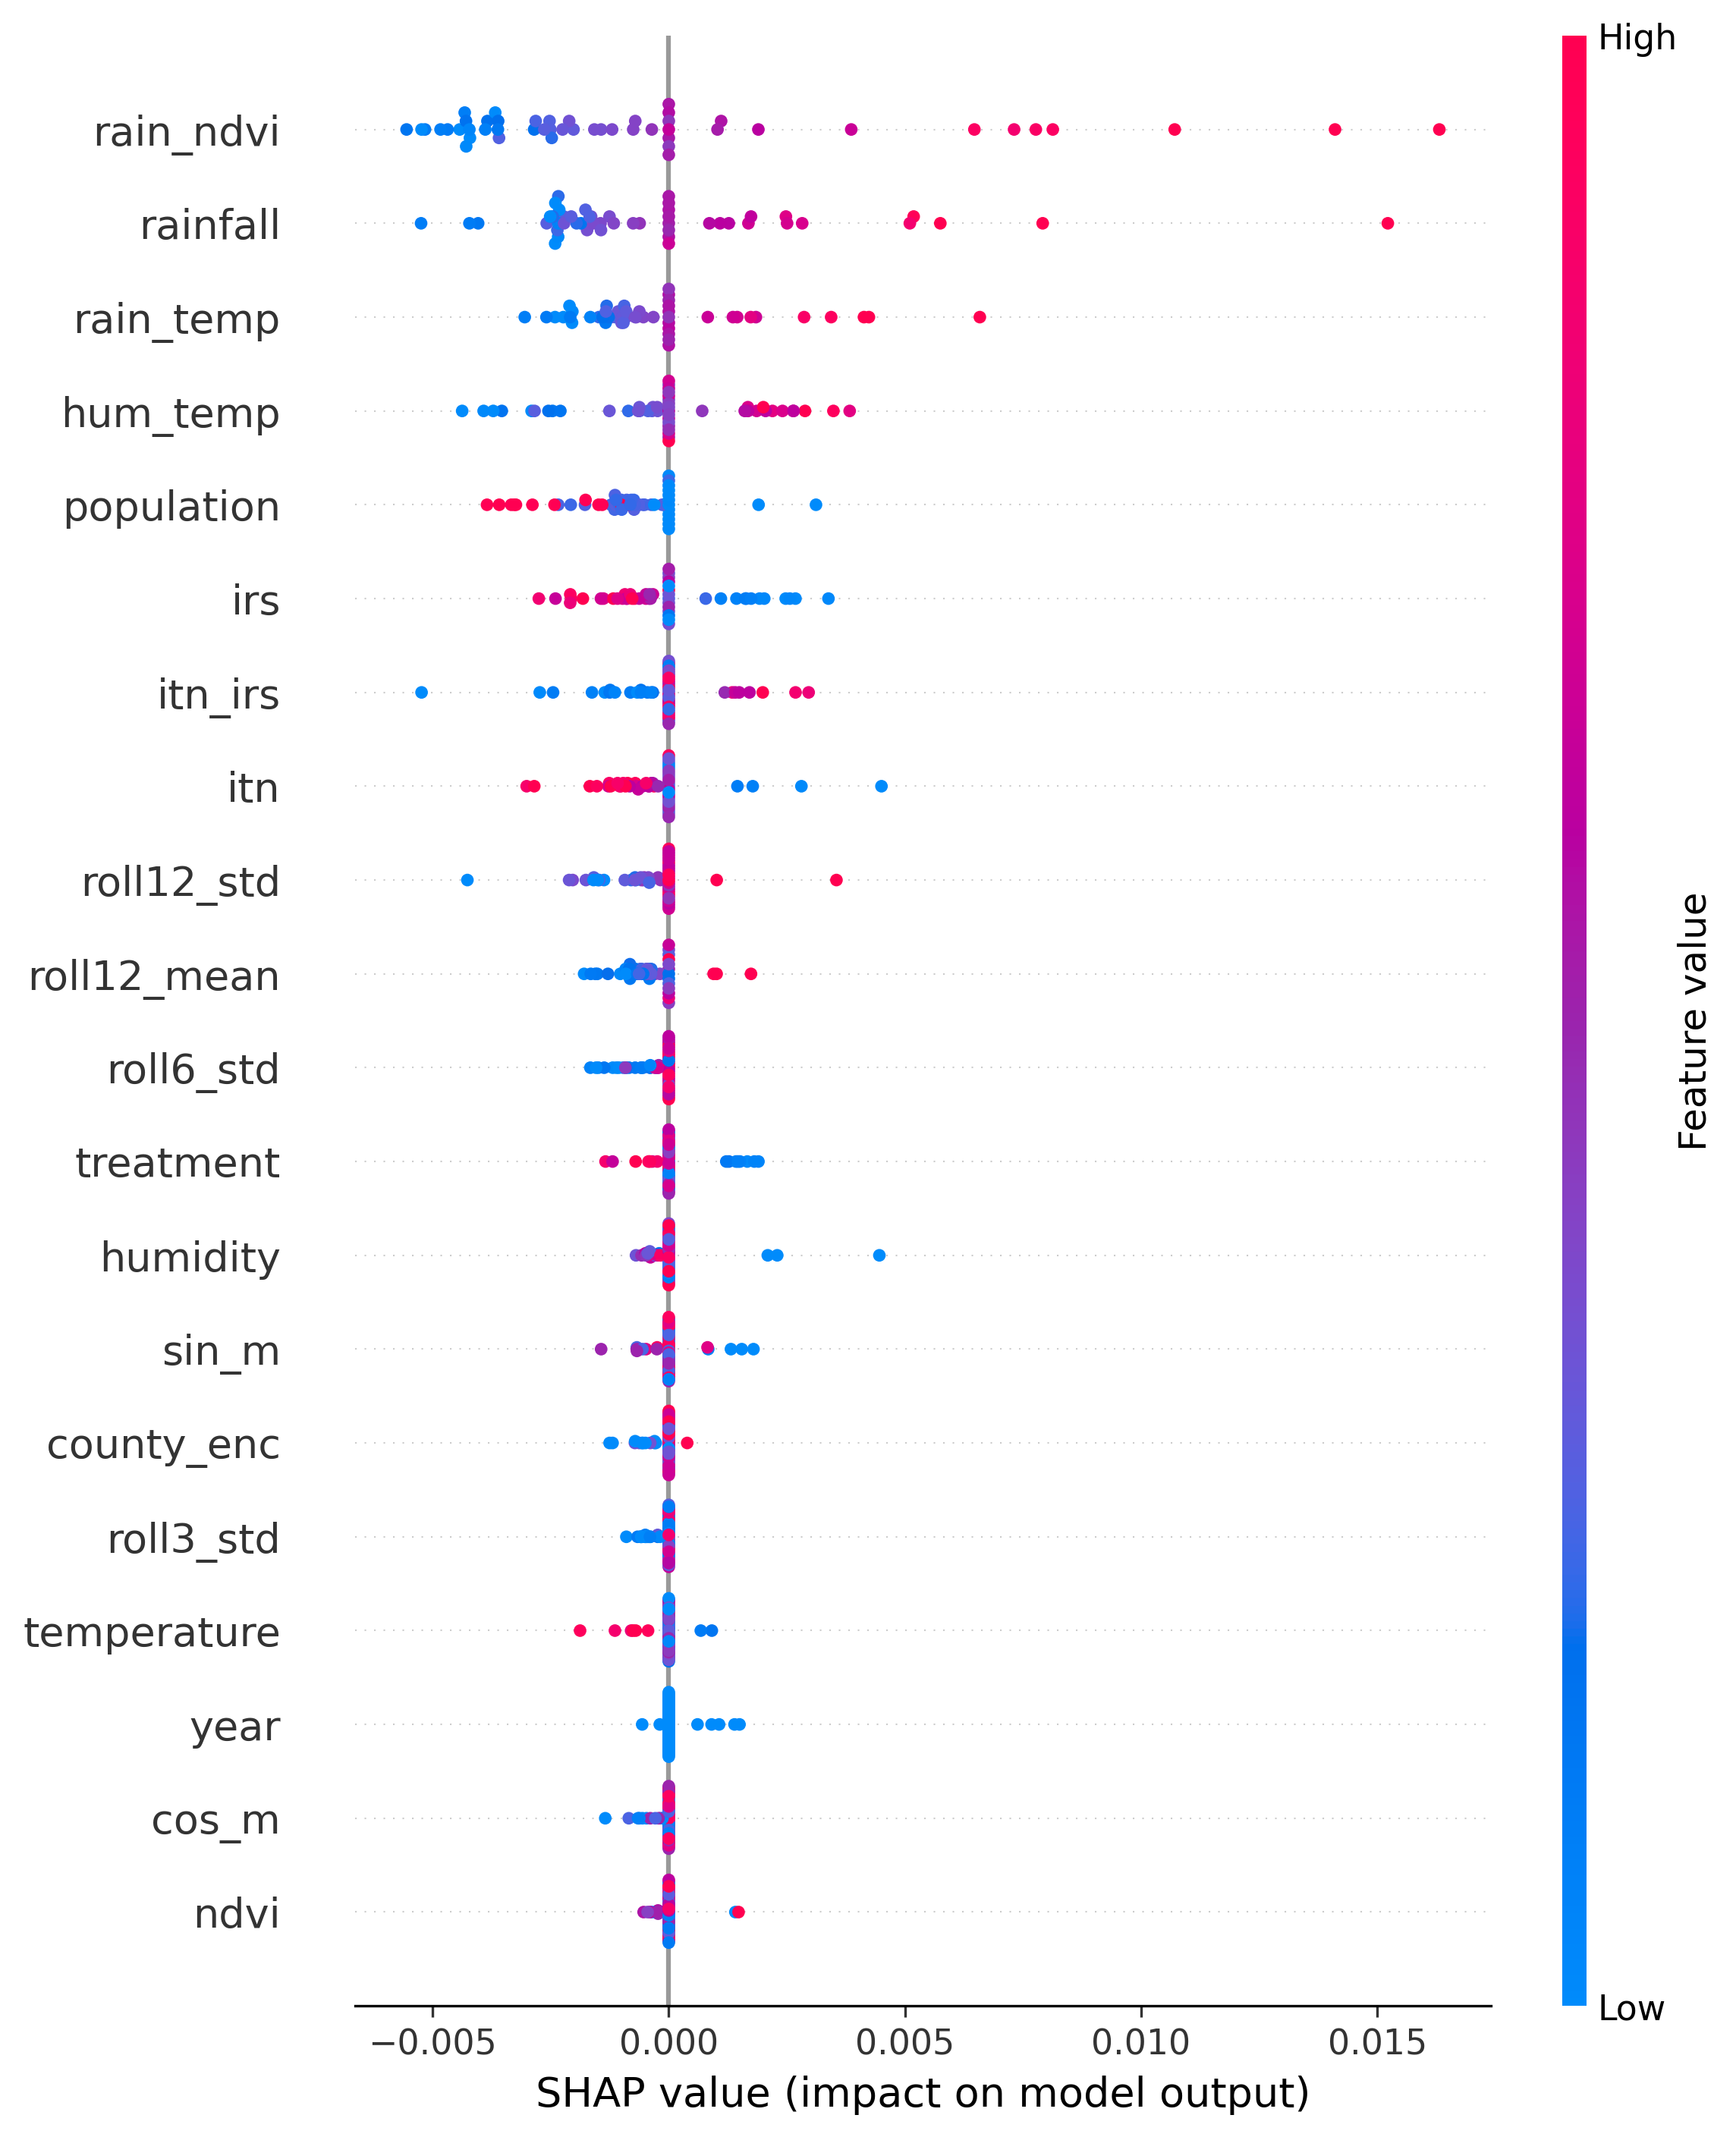
\includegraphics[width=0.52\textwidth]{ShapValues.png}
	\caption{SHAP Summary Plot of Predictor Variable Contributions}
	\label{fig:shap_summary}
\end{figure}

\vspace{-0.5cm}
 Figure \small  \ref{fig:shap_summary} presents the contribution of predictor variables to the model predictions. Variables positioned toward the right side(Red colors) of the plot were associated with increased malaria risk, while those on the left(blue color) were associated with lower predicted risk. 
Rainfall-related variables, including the rainfall-NDVI interaction, showed some of the largest positive SHAP values, suggesting that higher rainfall conditions were often associated with increased malaria risk. Temperature-humidity and rainfall-temperature interactions also contributed positively to the model predictions. On the other hand, higher coverage of interventions such as ITNs, IRS, and treatment access generally contributed toward lower predicted malaria risk. Overall, the results suggest that both environmental conditions and intervention measures play important roles in shaping malaria transmission patterns in Kenya.

\vspace{-0.5cm}
\section{Spatial Malaria Risk Mapping}

\begin{figure}[H]
	\centering
	
	\begin{minipage}[t]{0.32\textwidth}
		\centering
		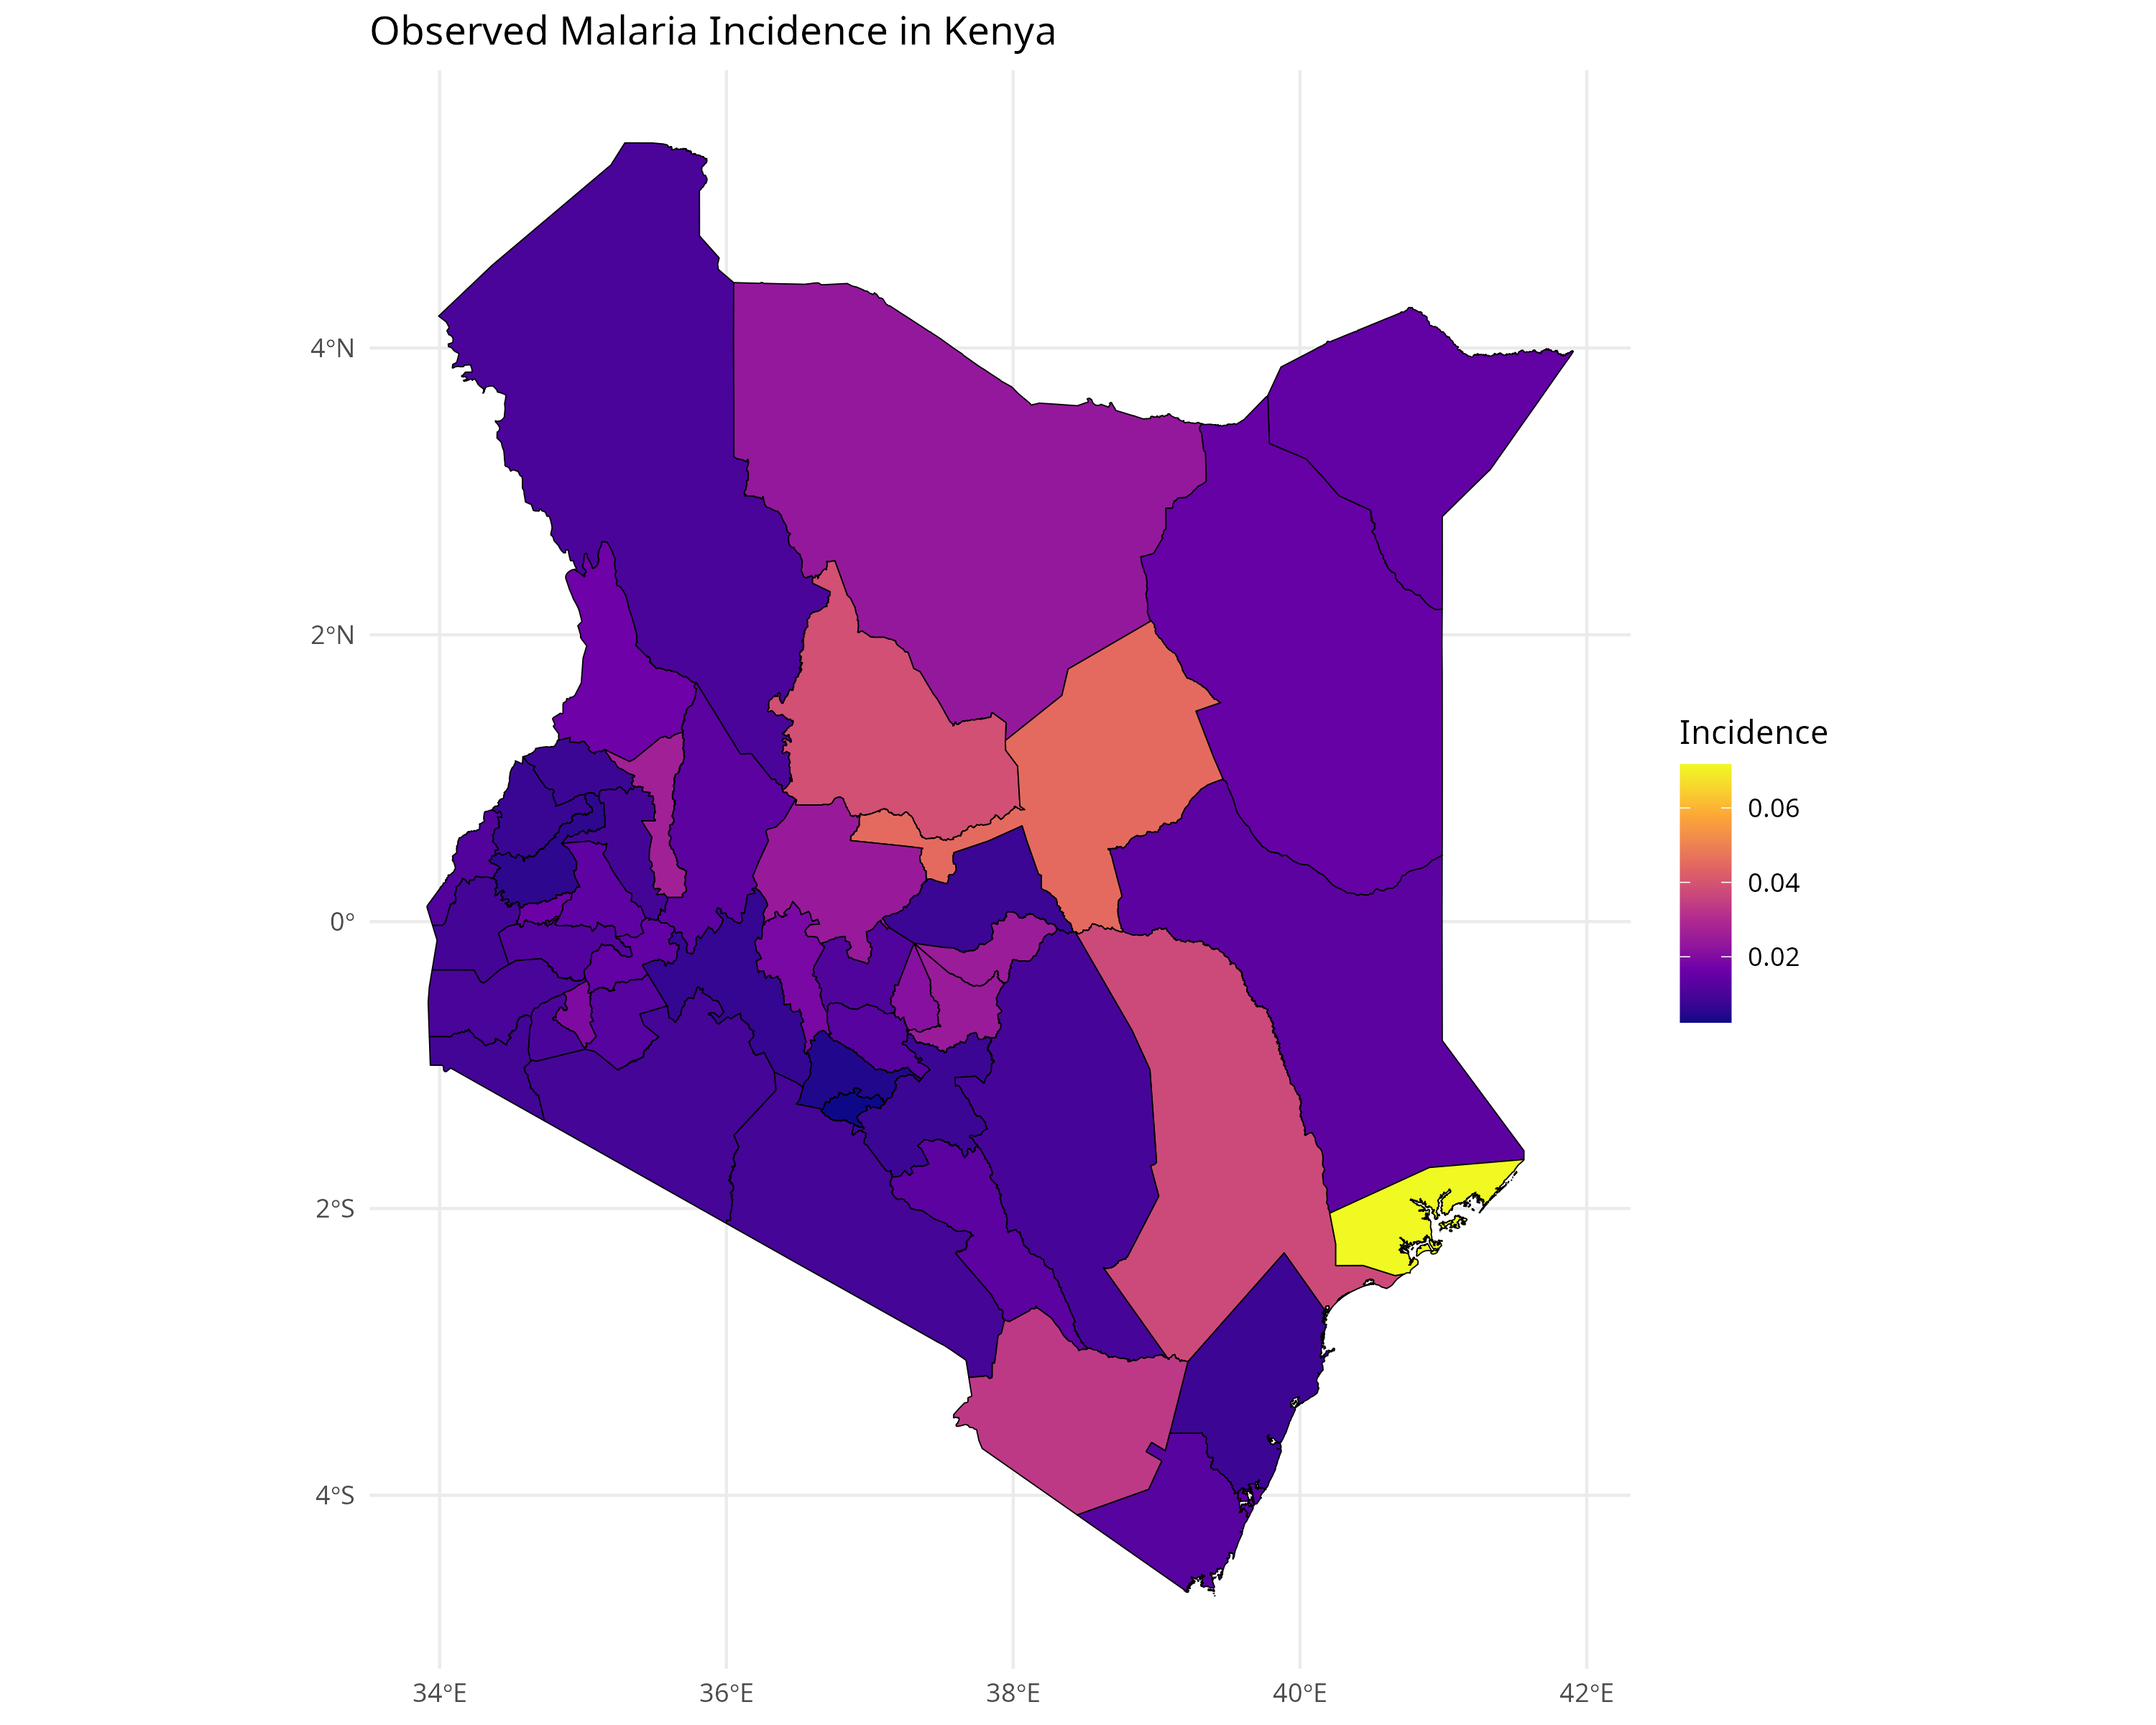
\includegraphics[width=\linewidth]{Observed_Malaria_Map.png}
		\caption*{(a) Observed Malaria Incidence}
	\end{minipage}
	\hfill
	\begin{minipage}[t]{0.32\textwidth}
		\centering
		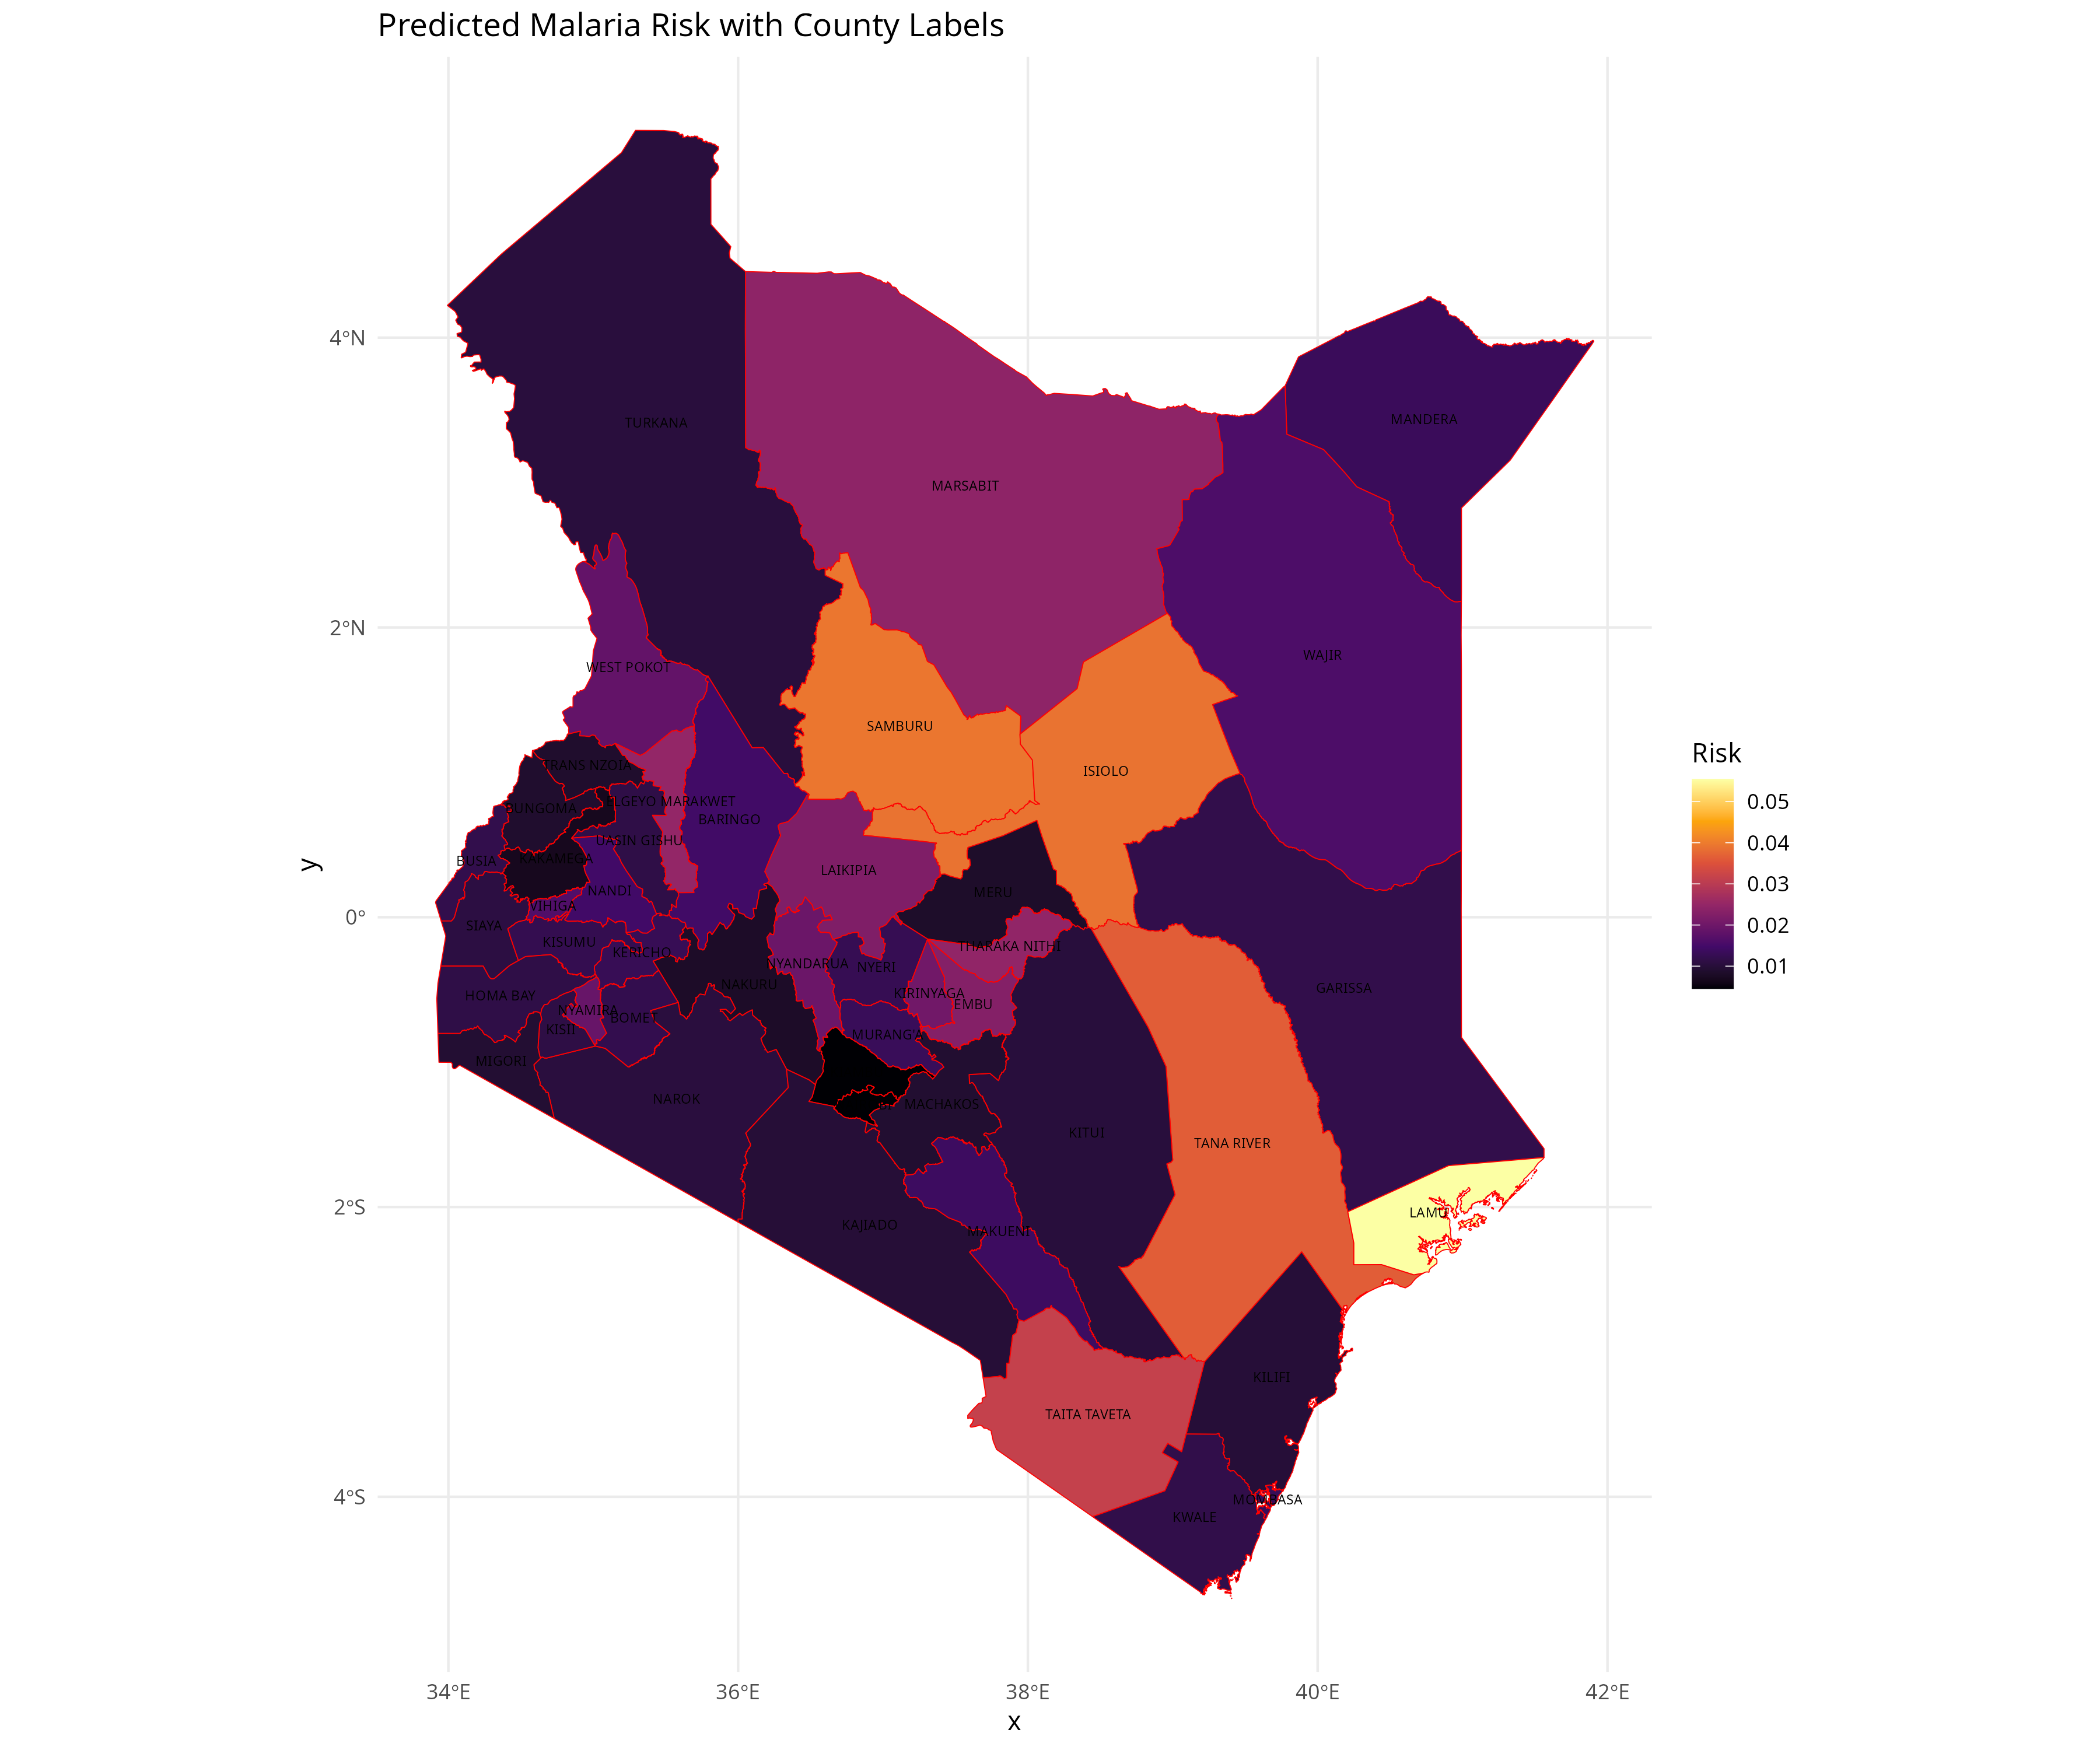
\includegraphics[width=\linewidth]{Predicted map labeled.png}
		\caption*{(b) Predicted Malaria Risk}
	\end{minipage}
	\hfill
	\begin{minipage}[t]{0.32\textwidth}
		\centering
		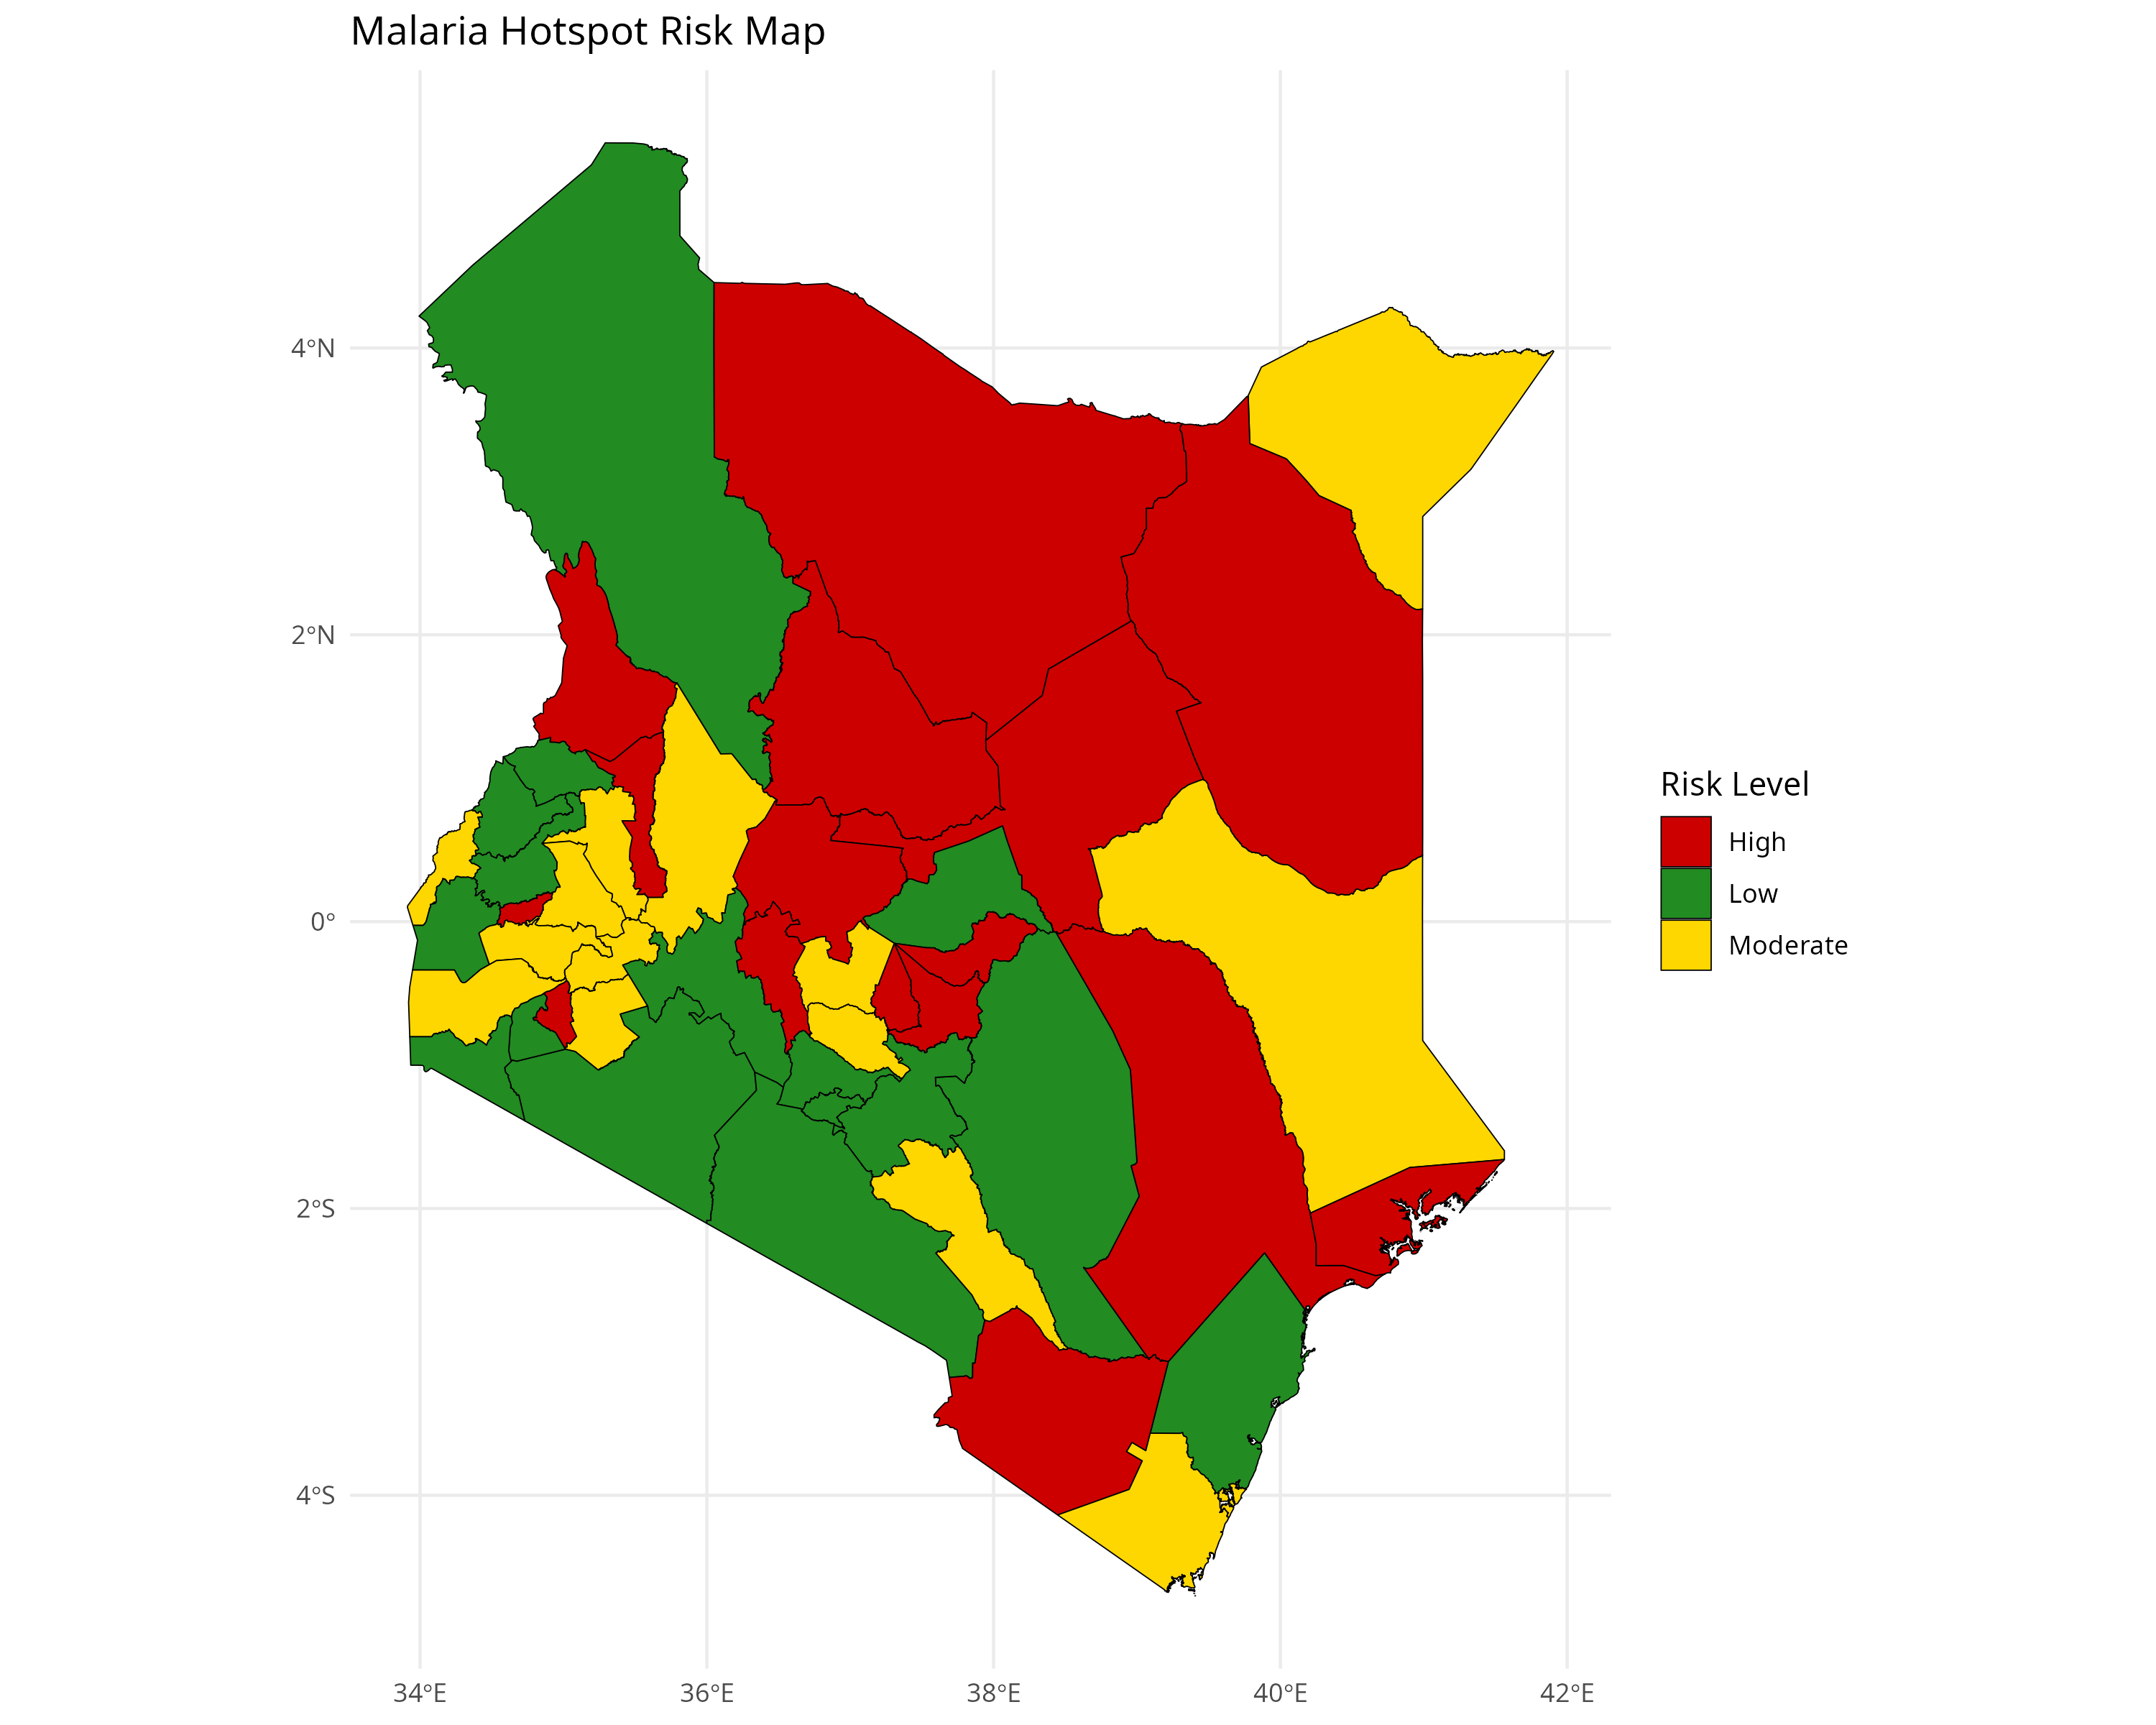
\includegraphics[width=\linewidth]{Hotspot_Risk_Map.png}
		\caption*{(c) Malaria Hotspot Classification}
	\end{minipage}
	
	\vspace{-0.2cm}
	
	\caption{Spatial Distribution of Observed and Predicted Malaria Risk Across Kenya}
	\label{fig:risk_mapping}
\end{figure}

\vspace{-0.3cm}

\small 
Figure \ref{fig:risk_mapping} illustrates the spatial distribution of observed malaria incidence, predicted malaria risk, and hotspot classifications across Kenya. The maps show clear geographical differences in malaria risk, indicating that malaria burden is not evenly distributed across the country. Higher malaria risk is evident in parts of the Lake Victoria basin and coastal region, while several counties in central Kenya exhibit relatively lower risk levels.

The hotspot classification map shows spatial differences by grouping counties into low, moderate, and high-risk categories. Counties such as  Isiolo, Tana River, and Lamu appear among the identified hotspots, whereas many central counties fall within the lower-risk categories. Overall, the results suggest that malaria risk is concentrated in specific regions of Kenya, providing useful information for targeted surveillance and intervention planning.

\section{Discussion}
Based on the results we found that both machine learning and hybrid deep learning models were able to predict malaria incidence across Kenyan counties using climatic, environmental, demographic, and intervention-related variables. The EDA analysis tells clear spatial and temporal variation in malaria transmission, particularly around the Lake Victoria basin and parts of the coastal region. This confirms the previous studies showing that malaria risk varies across ecological regions and seasons in Kenya \cite{amek2012spatial}.

Among the baseline models, XGBoost achieved the best predictive performance, with an $(R^2)$ value of 0.8202 and lower prediction errors than RF. These tells that XGBoost was more effective at capturing the nonlinear relationships between environmental conditions and malaria transmission. Similar observations have been reported in studies that applied ensemble tree-based methods to malaria forecasting \cite{Syafei2023}.

For the hybrid deep learning architectures, CNN-LSTM produced the best forecasting performance among the evaluated models. The model achieved lower RMSE and MAE values together with a high \(R^2\) value of 0.8096, indicating strong agreement between predicted and observed malaria incidence patterns. The forecasts also showed that CNN-LSTM was able to closely follow malaria transmission trends within hotspot counties such as Kisumu, Migori, Busia, and Lamu, although prediction differences became slightly larger during periods of unusually high malaria transmission.

The strong performance of CNN-LSTM is likely related to its hybrid architecture. The convolutional layers helped extract localized environmental patterns such as rainfall and vegetation interactions, while the LSTM component learned delayed temporal malaria trends across seasons and time periods. Compared to the standalone LSTM, CNN-GRU, and CNN-Transformer models, CNN-LSTM produced more stable forecasts with smaller prediction errors. In contrast, the weaker performance of the CNN-Transformer model may suggest that the available county-level dataset was not large enough for stable attention-based learning. This indicates that larger spatio-temporal datasets may further improve the performance of Transformer-based malaria forecasting models in future studies.

 Using SHAP analysis, we also found that rainfall, humidity, NDVI, and rainfall-related interaction variables were among the most influential predictors of malaria risk. Higher ITN, IRS, and treatment coverage were generally associated with lower predicted malaria risk. In addition, the malaria risk maps identified persistent hotspot areas, including Kisumu, Homa Bay, Busia, Lamu, and Taita Taveta, highlighting important geographical differences in malaria burden across Kenya.

Overall, our findings suggest that hybrid deep learning approaches, particularly CNN-LSTM, can provide useful support for malaria surveillance, hotspot detection, early warning systems, and targeted intervention planning in Kenya.
